\documentclass[letterpaper,11pt,notitlepage]{article}
% define the title
\usepackage{amsmath}
\usepackage{fixltx2e}
\usepackage{graphicx}
\usepackage[labelformat=empty]{caption}
\usepackage{subcaption}
\usepackage{listings}
\usepackage{color}
\usepackage{relsize}
\usepackage{wrapfig}
\usepackage{fontspec}
\usepackage{hyperref}
\usepackage{hanging}
\usepackage{textcomp,    % for \textlangle and \textrangle macros
            xspace}
\newcommand\la{\textlangle}  % set up short-form macros
\newcommand\ra{\textrangle\xspace}
\newcommand\rans{\textrangle}
\lstset{
  language={matlab},
  basicstyle=\ttfamily\smaller\relax,	
  tabsize=4,                              % Default tab size
  % showspaces=false,                       % Dont make spaces visible
  showtabs=false,                         % Dont make tabls visible
  columns=flexible,                       % Column formatc
  commentstyle=\color{mygreen}\textit,           % comment style
  extendedchars=true,              % lets you use non-ASCII characters; for 8-bits encodings only, does not work with UTF-8
  numbers=left,                    % where to put the line-numbers; possible values are (none, left, right)
  numbersep=8pt,                   % how far the line-numbers are from the code
  numberstyle=\tiny\color{mygray}, % the style that is used for the line-numbers
  stepnumber=1,
  xleftmargin=2cm,
  % backgroundcolor=\color{light-gray},
  breaklines=true,
  keywordstyle=\color{mynavy}
}
\hypersetup{colorlinks=true,linkcolor=blue}
\renewcommand*{\UrlFont}{\ttfamily\smaller\relax}

% \addtolength{\oddsidemargin}{0.5in}
% \addtolength{\evensidemargin}{0.5in}
% \addtolength{\textwidth}{-1in}
\addtolength{\topmargin}{-1in}
\addtolength{\textheight}{1.75in}
\setlength\parindent{24pt}

\definecolor{mygreen}{rgb}{0.1020,0.5961,0.3137}
\definecolor{mygray}{rgb}{0.5,0.5,0.5}
\definecolor{light-gray}{rgb}{0.8,0.8,0.8}
\definecolor{mynavy}{rgb}{0.1922,0.2118,0.5843}

\begin{document}

\begin{center}
	Homework 2 - LOGREG\\
	2015 Spring, Machine Learning\\
	Choong-Wan Woo\\
	\today\\
\end{center}

\hspace*{-1cm}\textbf{Analysis 1.}  \rule{10.5cm}{0.4pt}\\
\noindent\textit{What is the role of the learning rate?}\\

\noindent As shown in \textbf{Figure 1}, different step sizes (i.e., learning rates) have substantial influences on training and testing accuracy in stochastic gradient ascent of logistic regression models. The plots show large (e.g., 1.0) or small (e.g., 0.001) learning rates have negative effects on both training and testing accuracy. In our analysis, 0.1 or 0.01 showed high accuracy in both training and testing data. 

\begin{figure}[ht!]
	\centering
	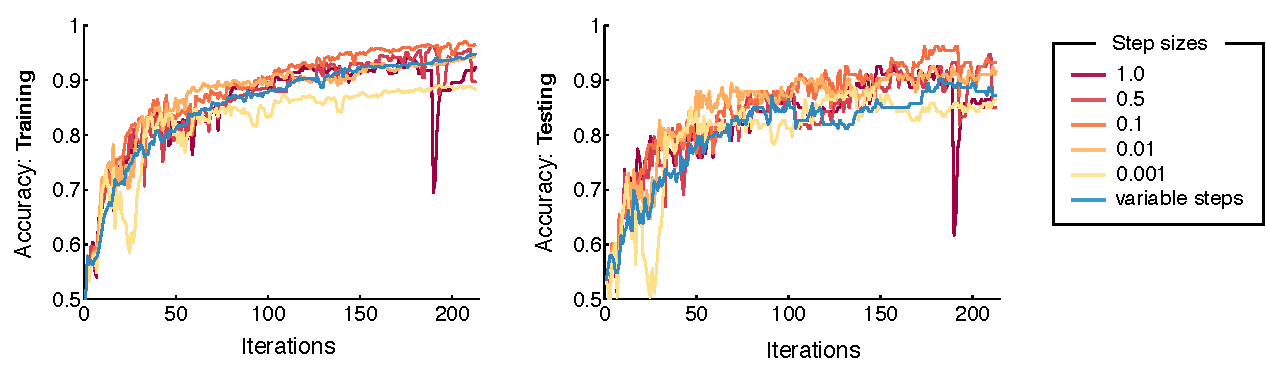
\includegraphics[width=12.5cm]{figure1_axis}
	\captionsetup{width=.8\textwidth}
	\caption{\textbf{Figure 1.} The effects of learning rate (i.e., step size of gradient ascent) on accuracy.} 
\end{figure}

\hspace*{-1cm}\textbf{Analysis 2.}  \rule{10.5cm}{0.4pt}\\
\noindent\textit{How many passes over the data do you need to complete?}\\

\noindent As \textbf{Figure 2} demonstrate, I tested one to five passes, and all of them seem okay given their high accuracy results. However, \textbf{Figure 2} shows an interesting pattern of results: The accuracy in training data kept increasing, whereas the accuracy in testing data decreased with five passes. Because this pattern could be due to an overfitting when five passes were used, four passes might be ideal.\\\\

\begin{figure}[ht!]
	\centering
	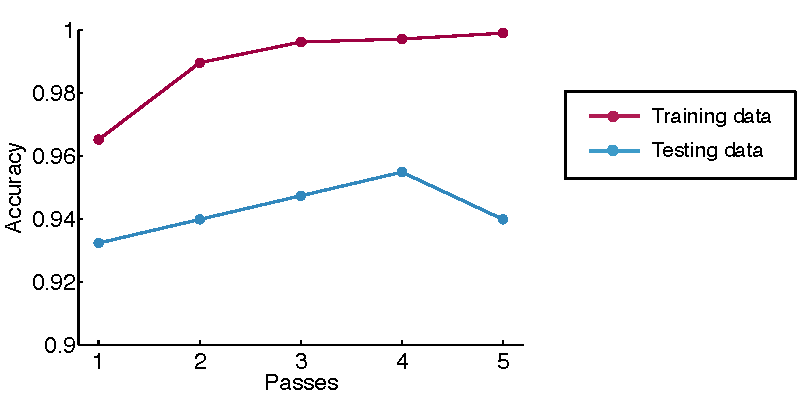
\includegraphics[width=9cm]{figure2_axis}
	\captionsetup{width=.8\textwidth}
	\caption{\textbf{Figure 2.} The effects of passes on accuracy.} 
\end{figure}

\hspace*{-1cm}\textbf{Analysis 3.}  \rule{10.5cm}{0.4pt}\\
\noindent\textit{What words are the best predictors of each class? How did you find them?}\\

\noindent From my analysis, the best predictor for the documents about baseball was \textbf{"hit"}, and the best predictor for hockey documents was \textbf{"hockey"}. To identify the best words, I found the words that have the maximum positive (for baseball) and negative (for hockey) beta values. What I mean by the maximum negative value is the biggest absolute value among the negative values.\\ 

\hspace*{-1cm}\textbf{Analysis 4.}  \rule{10.5cm}{0.4pt}\\
\noindent\textit{What words are the poorest predictors of classes? How did you find them?}\\

\noindent The poorest predictor for the documents about baseball was \textbf{"tandem"}, and the poorest predictor for hockey documents was \textbf{"kicked"}. To identify the poorest words, I searched the words that have the minimum positive (for baseball) and negative (for hockey) beta values. What I mean by the minimum negative value is the smallest absolute value among negative values.\\

\hspace*{-1cm}\textbf{Extra.}  \rule{10.5cm}{0.4pt}\\
\noindent\textit{Use a schedule to update the learning rate, and show the effect in your analysis document}\\

\noindent In my submission of \textbf{logreg.py}, I used $\frac{2}{\sqrt{iteration}}$ to update the learning rate over iterations (which is activated by adding the argument, \textbf{\--\--var\_step True}
). The results of using the argument are shown in \textbf{Figure 1} using a blue line. In  The results were not better than a fixed learning rate (e.g., 0.1). 

\end{document}